
Generated: 2026-02-06 21:26


\chapter{1. Objective}

Minimize cooling-tower lateral shell area using SA, PSO, and BFGS while enforcing fixed target volume and scenario-specific constructability constraints.

The study compares stochastic and deterministic optimization behavior across eight structurally different problem setups while keeping common engineering requirements (capacity and realistic shape) explicit in the objective.


\chapter{2. Geometry Model}

The tower is modeled as a stack of frustums.


\begin{itemize}
\item Frustum area: \texttt{A\_i = pi * (r\_\{i-1\} + r\_i) * sqrt((r\_i - r\_\{i-1\})\textasciicircum{}2 + h\_i\textasciicircum{}2)}
\item Frustum volume: \texttt{V\_i = (pi * h\_i / 3) * (r\_\{i-1\}\textasciicircum{}2 + r\_\{i-1\}*r\_i + r\_i\textasciicircum{}2)}
\item Tower totals: \texttt{A = sum(A\_i)}, \texttt{V = sum(V\_i)}
\end{itemize}

Lateral shell area is optimized (top and bottom caps excluded), which directly corresponds to shell-construction material for fixed end radii.

Analytic gradients were used for both \texttt{A} and \texttt{V}, and for all penalty terms, so BFGS receives exact first-order information.


\section{2.1 Design Variables by Scenario Type}

\begin{itemize}
\item \texttt{radii} mode: optimize interior radii \texttt{r1..r\_\{m-1\}} while ring heights are fixed from \texttt{z} levels.
\item \texttt{heights} mode: optimize segment heights \texttt{h1..hm} while all ring radii are fixed.
\item \texttt{joint} mode: optimize both interior radii and all heights simultaneously.
\end{itemize}

\chapter{3. Optimization Methods}


\section{3.1 Simulated Annealing (SA)}

SA performs single-solution stochastic search. At each evaluation, a local perturbation is proposed and accepted if it improves objective, or probabilistically accepted otherwise using the temperature schedule.

This supports escape from local minima early in search and gradual exploitation as temperature cools.


\section{3.2 Particle Swarm Optimization (PSO)}

PSO evolves a population of particles with velocity updates using inertia, cognitive pull to personal best, and social pull to global best.

It is typically strong on global exploration and multimodal landscapes, but can require many evaluations to satisfy strict constraints.


\section{3.3 BFGS (Deterministic Quasi-Newton)}

BFGS updates an inverse-Hessian approximation and computes descent directions with line search, yielding rapid local convergence when gradients are informative.

It is efficient in evaluation count but can be sensitive to initialization and non-convex penalties.


\chapter{4. Penalized Objective and Geometrical Constraints}

The optimized scalar objective is \texttt{J(x) = A(x) + P\_volume + P\_height + P\_shape + P\_smooth + P\_bounds + P\_ratio} (terms enabled per scenario).


\section{4.1 Constraint Terms and Their Function}

\begin{itemize}
\item \texttt{P\_volume}: enforces target cooling capacity by penalizing relative deviation from target volume.
\item \texttt{P\_height}: enforces total tower height in scenarios where heights vary, preserving comparable overall structure.
\item \texttt{P\_shape}: enforces hyperboloid-like monotonic contraction to neck and expansion above neck.
\item \texttt{P\_smooth}: penalizes second differences in radii to avoid oscillatory/sawtooth shell profiles.
\item \texttt{P\_bounds}: hinge penalty for design-variable bounds to keep variables in practical/constructable ranges.
\item \texttt{P\_ratio} (S8): limits adjacent-height ratios to promote constructability and avoid abrupt segment transitions.
\end{itemize}

\section{4.2 Feasibility Rule}

\begin{itemize}
\item Relative volume error must be \texttt{<= 1e-3}.
\item If heights vary, relative total-height error must be \texttt{<= 1e-3}.
\item If radii vary, monotonic hyperboloid violation must be \texttt{<= 1e-6}.
\end{itemize}

\chapter{5. Optimization Protocol}

\begin{itemize}
\item Runs per algorithm per scenario: 10
\item Seed offset: 0
\item SA: \texttt{temp\_init=120}, \texttt{cooling\_rate=0.997}, scenario-dependent \texttt{step\_size}
\item PSO: \texttt{w=0.65}, \texttt{c1=1.6}, \texttt{c2=1.7}, particles = 40 or 50 by dimension
\item BFGS: \texttt{tol=1e-7}, \texttt{max\_iter=1200}
\item Penalties: volume, height sum (when applicable), shape monotonicity, smoothness, bounds, ratio (S8)
\end{itemize}

Stochastic budgets are 10k evaluations for lower-dimensional setups and 16k for joint/high-dimensional setups. BFGS uses smaller budgets due to faster local convergence.


\chapter{6. Scenario Definitions}

\begin{longtable}{p{0.13\textwidth} | p{0.13\textwidth} | p{0.13\textwidth} | p{0.13\textwidth} | p{0.13\textwidth} | p{0.13\textwidth} | p{0.13\textwidth}}
\hline
ID & Mode & m & Target Volume & r0 & rm & Description \\
\hline
\endfirsthead
\hline
ID & Mode & m & Target Volume & r0 & rm & Description \\
\hline
\endhead
S1 & radii & 10 & 70320 & 39.3 & 27.4 & Required case with bounded radii and required ring heights. \\
S2 & radii & 10 & 70320 & 39.3 & 27.4 & Required case with wide radii range (unconstrained-like). \\
S3 & radii & 10 & 70320 & 39.3 & 27.4 & Uniform-height radii design with bounded radii. \\
S4 & radii & 12 & 70320 & 39.3 & 27.4 & Finer discretization (m=12) with bounded radii and smoothness. \\
S5 & heights & 10 & 70320 & 39.3 & 27.4 & Fixed radii, optimize bounded heights. \\
S6 & heights & 10 & 70320 & 39.3 & 27.4 & Fixed radii, optimize wide-range heights (unconstrained-like). \\
S7 & joint & 10 & 70320 & 39.3 & 27.4 & Joint bounded optimization of radii and heights. \\
S8 & joint & 10 & 90000 & 39.3 & 27.4 & Joint constructability-aware design with larger target volume. \\
\hline
\end{longtable}


\chapter{7. Cross-Algorithm Summary}

\begin{longtable}{p{0.13\textwidth} | p{0.13\textwidth} | p{0.13\textwidth} | p{0.13\textwidth} | p{0.13\textwidth} | p{0.13\textwidth} | p{0.13\textwidth}}
\hline
Algorithm & Total Runs & Mean Area & Mean Rel Vol Err & Mean Evals & Mean Time (s) & Feasibility Rate \\
\hline
\endfirsthead
\hline
Algorithm & Total Runs & Mean Area & Mean Rel Vol Err & Mean Evals & Mean Time (s) & Feasibility Rate \\
\hline
\endhead
SA & 80 & 7814.56 & 5.277e-04 & 11500.0 & 0.5448 & 71.2\% \\
PSO & 80 & 8264.80 & 1.698e-02 & 11500.0 & 0.5803 & 50.0\% \\
BFGS & 80 & 7850.64 & 4.018e-04 & 4227.9 & 0.2061 & 72.5\% \\
\hline
\end{longtable}


\begin{figure}[H]
\centering

\includegraphics[width=0.95\textwidth]{../results/figures/cross_scenario_area_bar.png}
\caption{Cross-scenario area comparison}
\end{figure}


\chapter{8. Scenario Results}


\section{S1}

\begin{longtable}{p{0.13\textwidth} | p{0.13\textwidth} | p{0.13\textwidth} | p{0.13\textwidth} | p{0.13\textwidth} | p{0.13\textwidth} | p{0.13\textwidth}}
\hline
Algorithm & Mean Area & Std Area & Mean Rel Vol Err & Mean Evals & Mean Time (s) & Feasibility Rate \\
\hline
\endfirsthead
\hline
Algorithm & Mean Area & Std Area & Mean Rel Vol Err & Mean Evals & Mean Time (s) & Feasibility Rate \\
\hline
\endhead
BFGS & 7782.01 & 0.00 & 1.537e-03 & 3302.6 & 0.1651 & 0.0\% \\
PSO & 7950.10 & 201.50 & 1.571e-02 & 10000.0 & 0.5382 & 20.0\% \\
SA & 7781.85 & 4.69 & 1.246e-03 & 10000.0 & 0.5088 & 50.0\% \\
\hline
\end{longtable}


\begin{figure}[H]
\centering

\includegraphics[width=0.95\textwidth]{../results/figures/S1_convergence.png}
\caption{S1 convergence}
\end{figure}


\begin{figure}[H]
\centering

\includegraphics[width=0.95\textwidth]{../results/figures/S1_profile_overlay.png}
\caption{S1 profile}
\end{figure}


\begin{figure}[H]
\centering
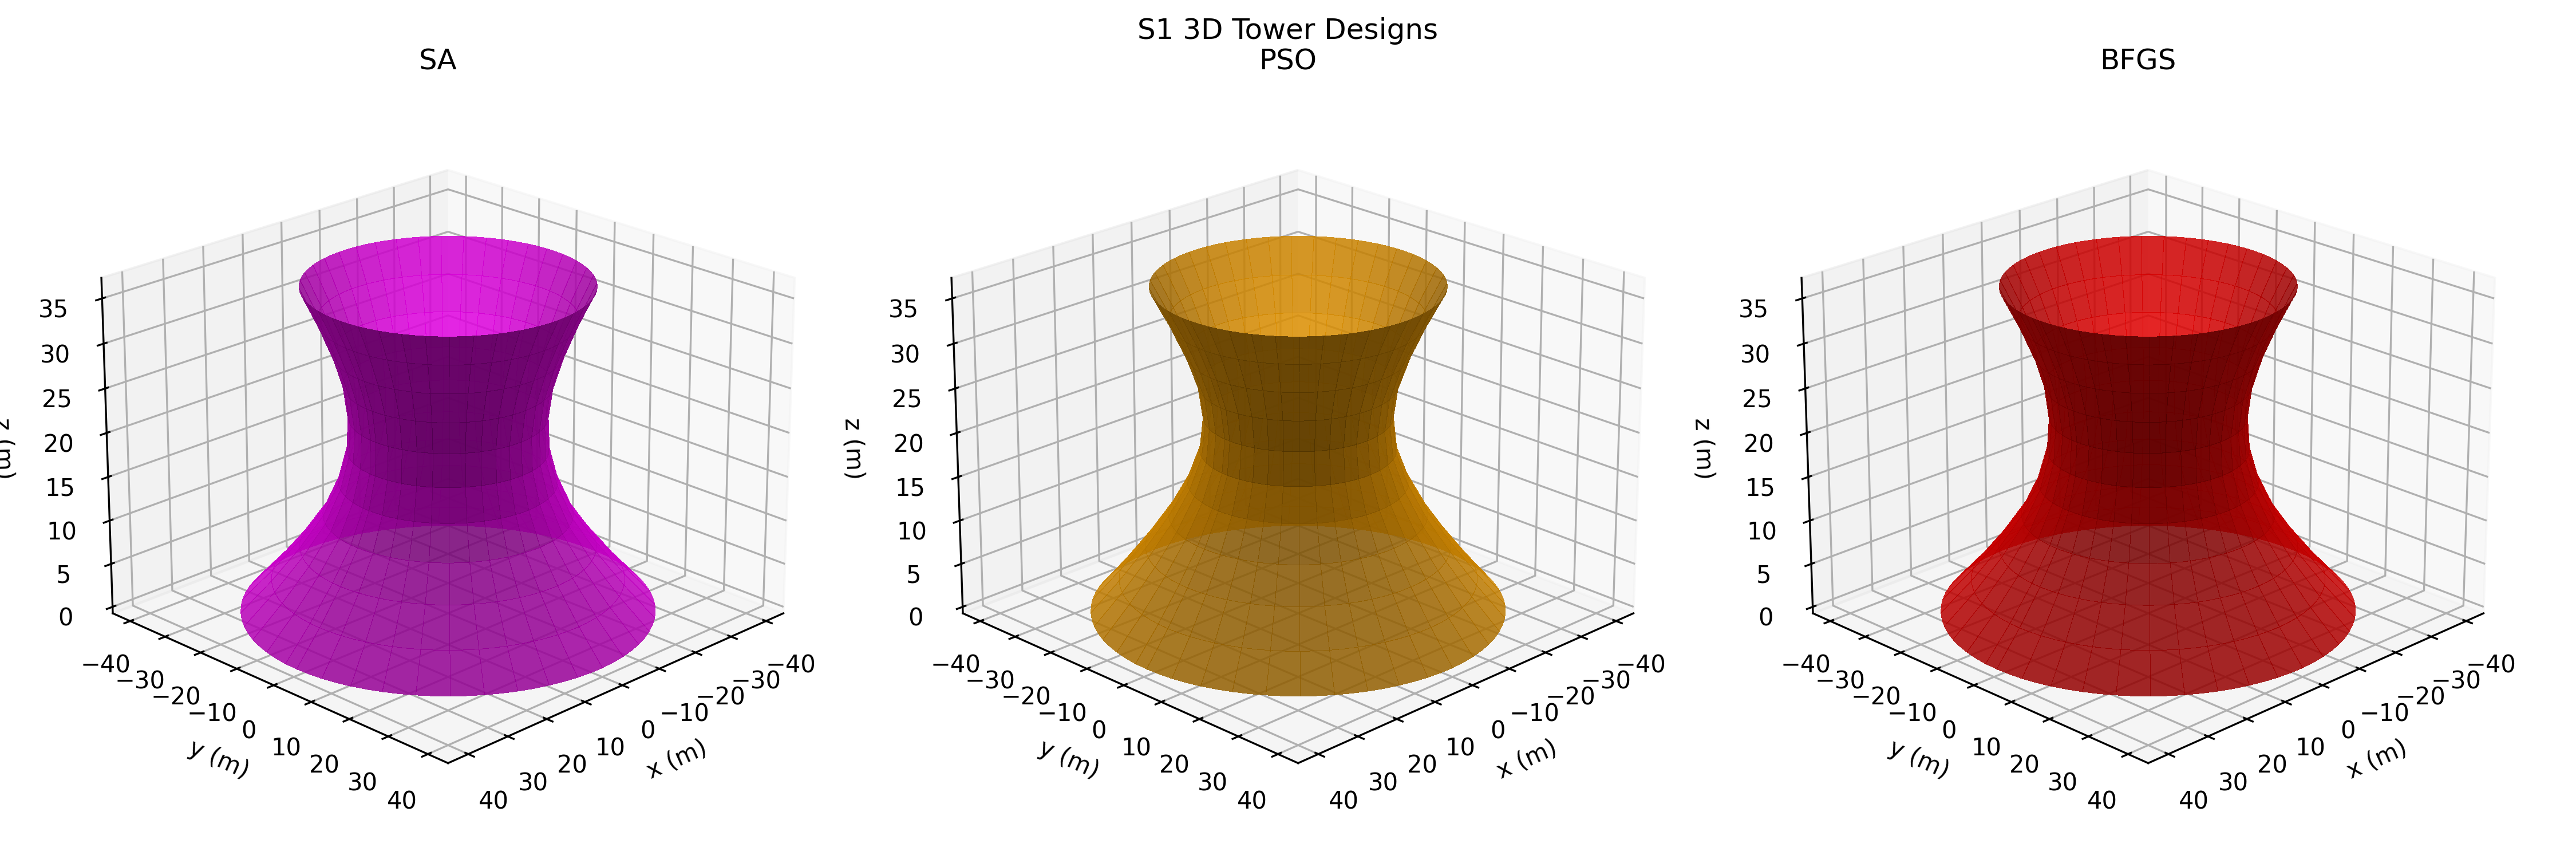
\includegraphics[width=0.95\textwidth]{../results/figures/S1_tower_3d.png}
\caption{S1 3D towers}
\end{figure}



\section{S2}

\begin{longtable}{p{0.13\textwidth} | p{0.13\textwidth} | p{0.13\textwidth} | p{0.13\textwidth} | p{0.13\textwidth} | p{0.13\textwidth} | p{0.13\textwidth}}
\hline
Algorithm & Mean Area & Std Area & Mean Rel Vol Err & Mean Evals & Mean Time (s) & Feasibility Rate \\
\hline
\endfirsthead
\hline
Algorithm & Mean Area & Std Area & Mean Rel Vol Err & Mean Evals & Mean Time (s) & Feasibility Rate \\
\hline
\endhead
BFGS & 8051.30 & 532.40 & 1.485e-04 & 3945.5 & 0.1574 & 100.0\% \\
PSO & 9352.84 & 524.78 & 6.536e-02 & 10000.0 & 0.4444 & 40.0\% \\
SA & 7753.26 & 9.27 & 5.492e-05 & 10000.0 & 0.4173 & 100.0\% \\
\hline
\end{longtable}


\begin{figure}[H]
\centering

\includegraphics[width=0.95\textwidth]{../results/figures/S2_convergence.png}
\caption{S2 convergence}
\end{figure}


\begin{figure}[H]
\centering

\includegraphics[width=0.95\textwidth]{../results/figures/S2_profile_overlay.png}
\caption{S2 profile}
\end{figure}


\begin{figure}[H]
\centering
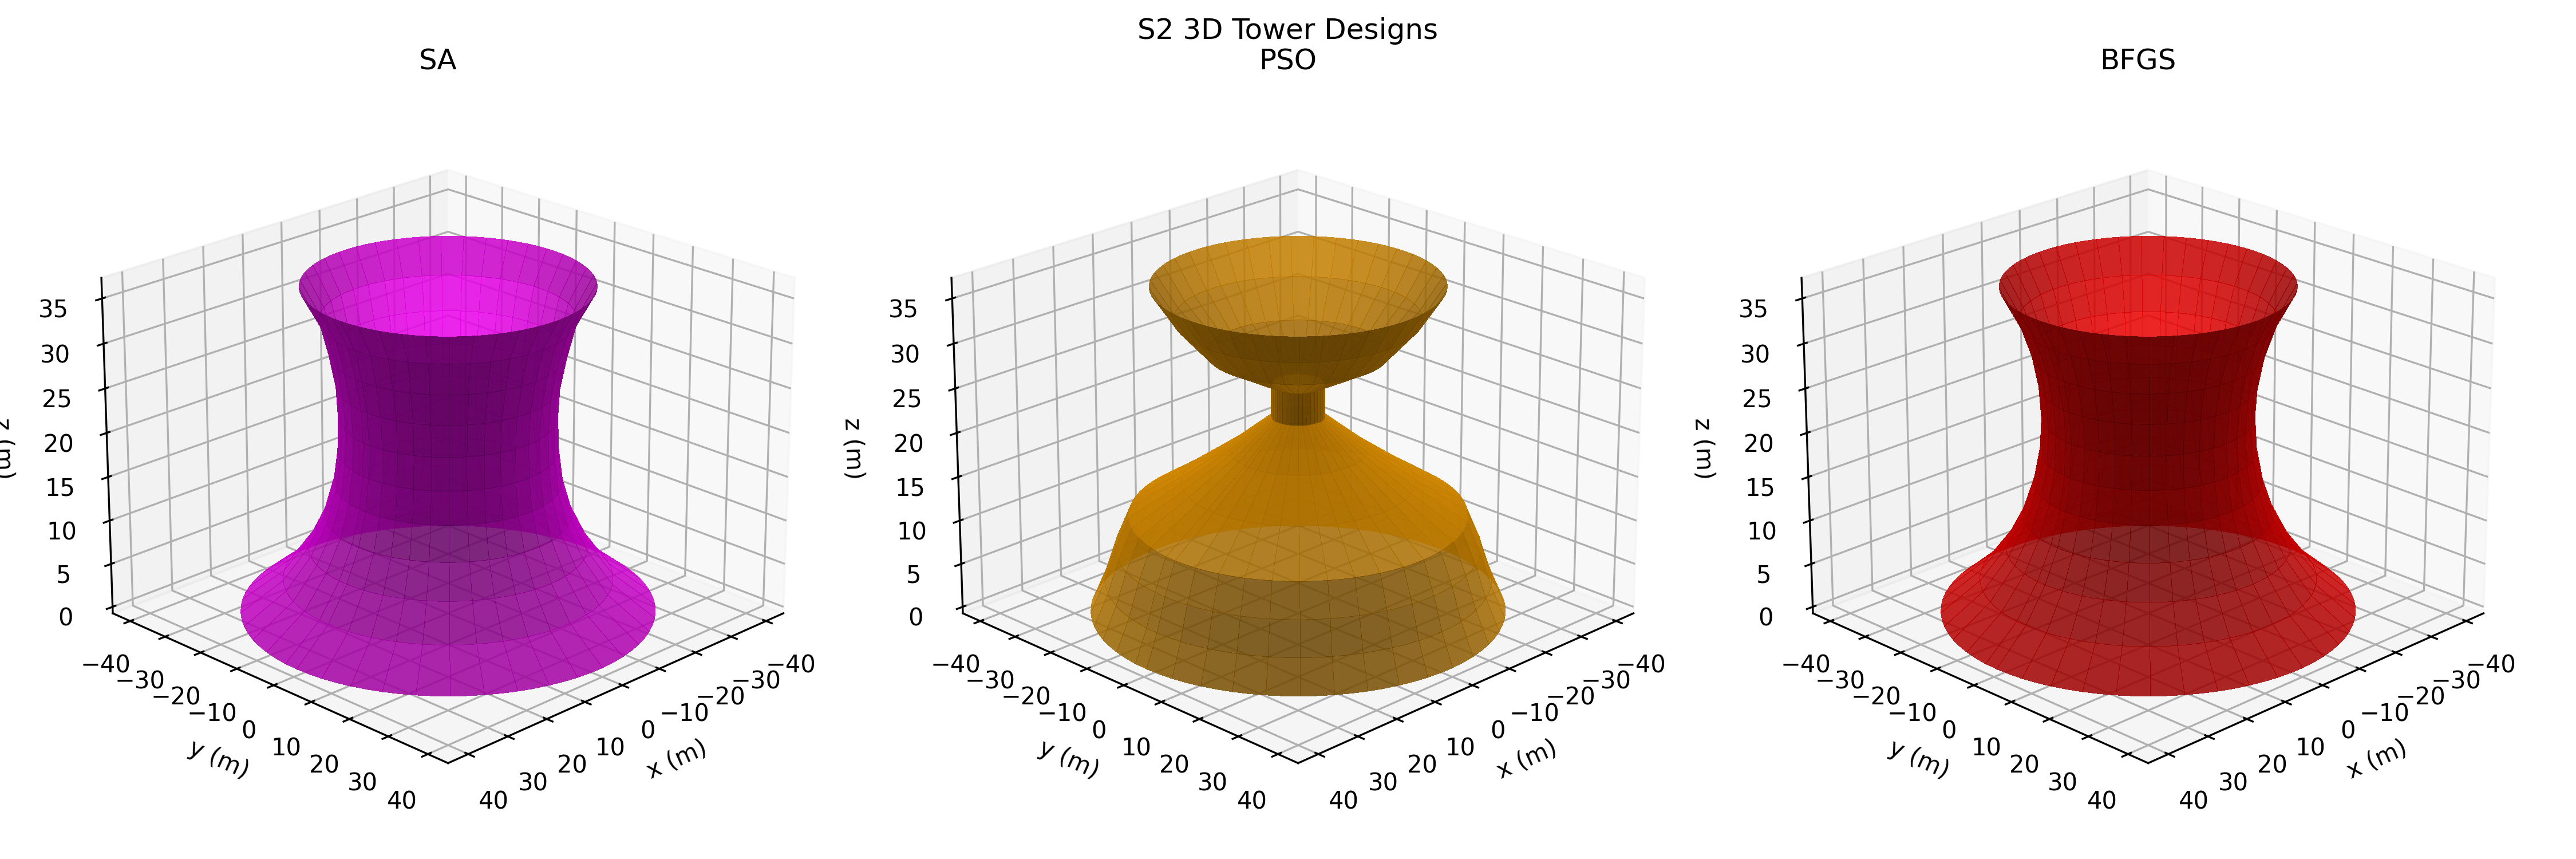
\includegraphics[width=0.95\textwidth]{../results/figures/S2_tower_3d.png}
\caption{S2 3D towers}
\end{figure}



\section{S3}

\begin{longtable}{p{0.13\textwidth} | p{0.13\textwidth} | p{0.13\textwidth} | p{0.13\textwidth} | p{0.13\textwidth} | p{0.13\textwidth} | p{0.13\textwidth}}
\hline
Algorithm & Mean Area & Std Area & Mean Rel Vol Err & Mean Evals & Mean Time (s) & Feasibility Rate \\
\hline
\endfirsthead
\hline
Algorithm & Mean Area & Std Area & Mean Rel Vol Err & Mean Evals & Mean Time (s) & Feasibility Rate \\
\hline
\endhead
BFGS & 7926.31 & 300.48 & 1.541e-04 & 2904.7 & 0.1189 & 100.0\% \\
PSO & 8258.12 & 351.80 & 2.509e-05 & 10000.0 & 0.4407 & 90.0\% \\
SA & 7753.02 & 21.36 & 3.424e-05 & 10000.0 & 0.4156 & 100.0\% \\
\hline
\end{longtable}


\begin{figure}[H]
\centering

\includegraphics[width=0.95\textwidth]{../results/figures/S3_convergence.png}
\caption{S3 convergence}
\end{figure}


\begin{figure}[H]
\centering
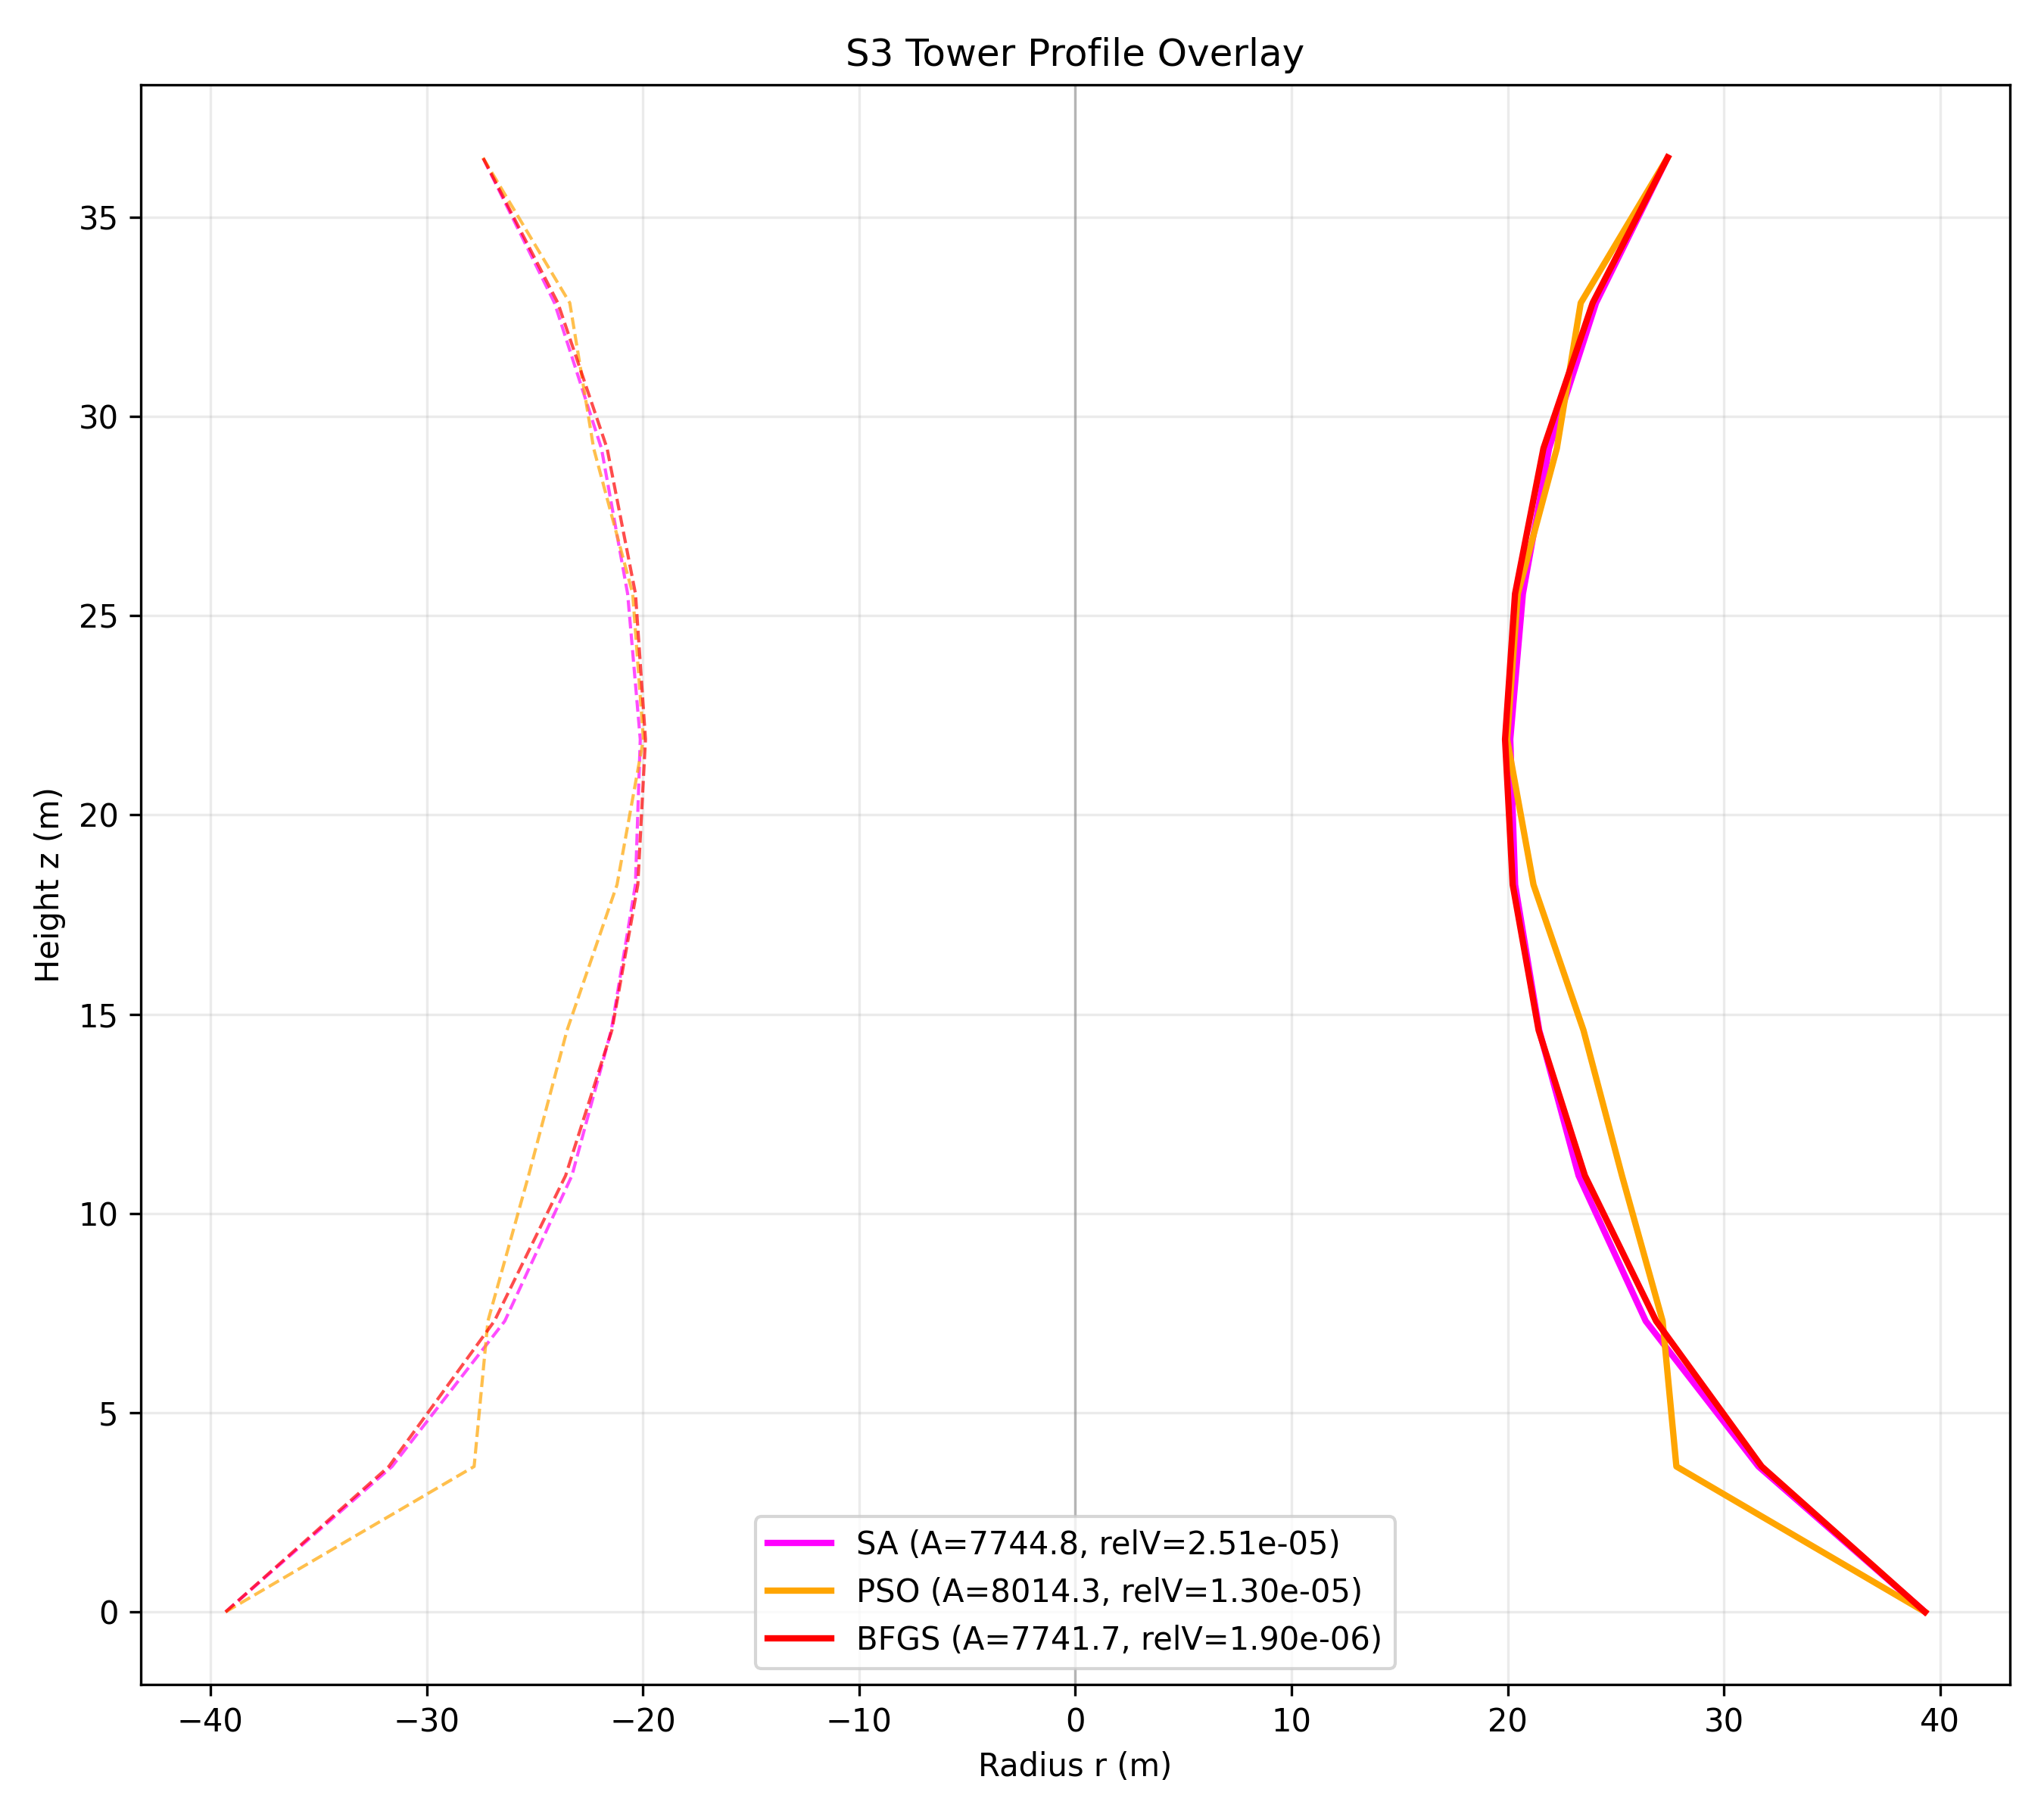
\includegraphics[width=0.95\textwidth]{../results/figures/S3_profile_overlay.png}
\caption{S3 profile}
\end{figure}


\begin{figure}[H]
\centering

\includegraphics[width=0.95\textwidth]{../results/figures/S3_tower_3d.png}
\caption{S3 3D towers}
\end{figure}



\section{S4}

\begin{longtable}{p{0.13\textwidth} | p{0.13\textwidth} | p{0.13\textwidth} | p{0.13\textwidth} | p{0.13\textwidth} | p{0.13\textwidth} | p{0.13\textwidth}}
\hline
Algorithm & Mean Area & Std Area & Mean Rel Vol Err & Mean Evals & Mean Time (s) & Feasibility Rate \\
\hline
\endfirsthead
\hline
Algorithm & Mean Area & Std Area & Mean Rel Vol Err & Mean Evals & Mean Time (s) & Feasibility Rate \\
\hline
\endhead
BFGS & 7779.85 & 0.00 & 8.915e-04 & 4101.4 & 0.2142 & 100.0\% \\
PSO & 8269.55 & 447.60 & 3.272e-02 & 10000.0 & 0.5666 & 0.0\% \\
SA & 7783.18 & 14.88 & 1.557e-03 & 10000.0 & 0.5289 & 20.0\% \\
\hline
\end{longtable}


\begin{figure}[H]
\centering
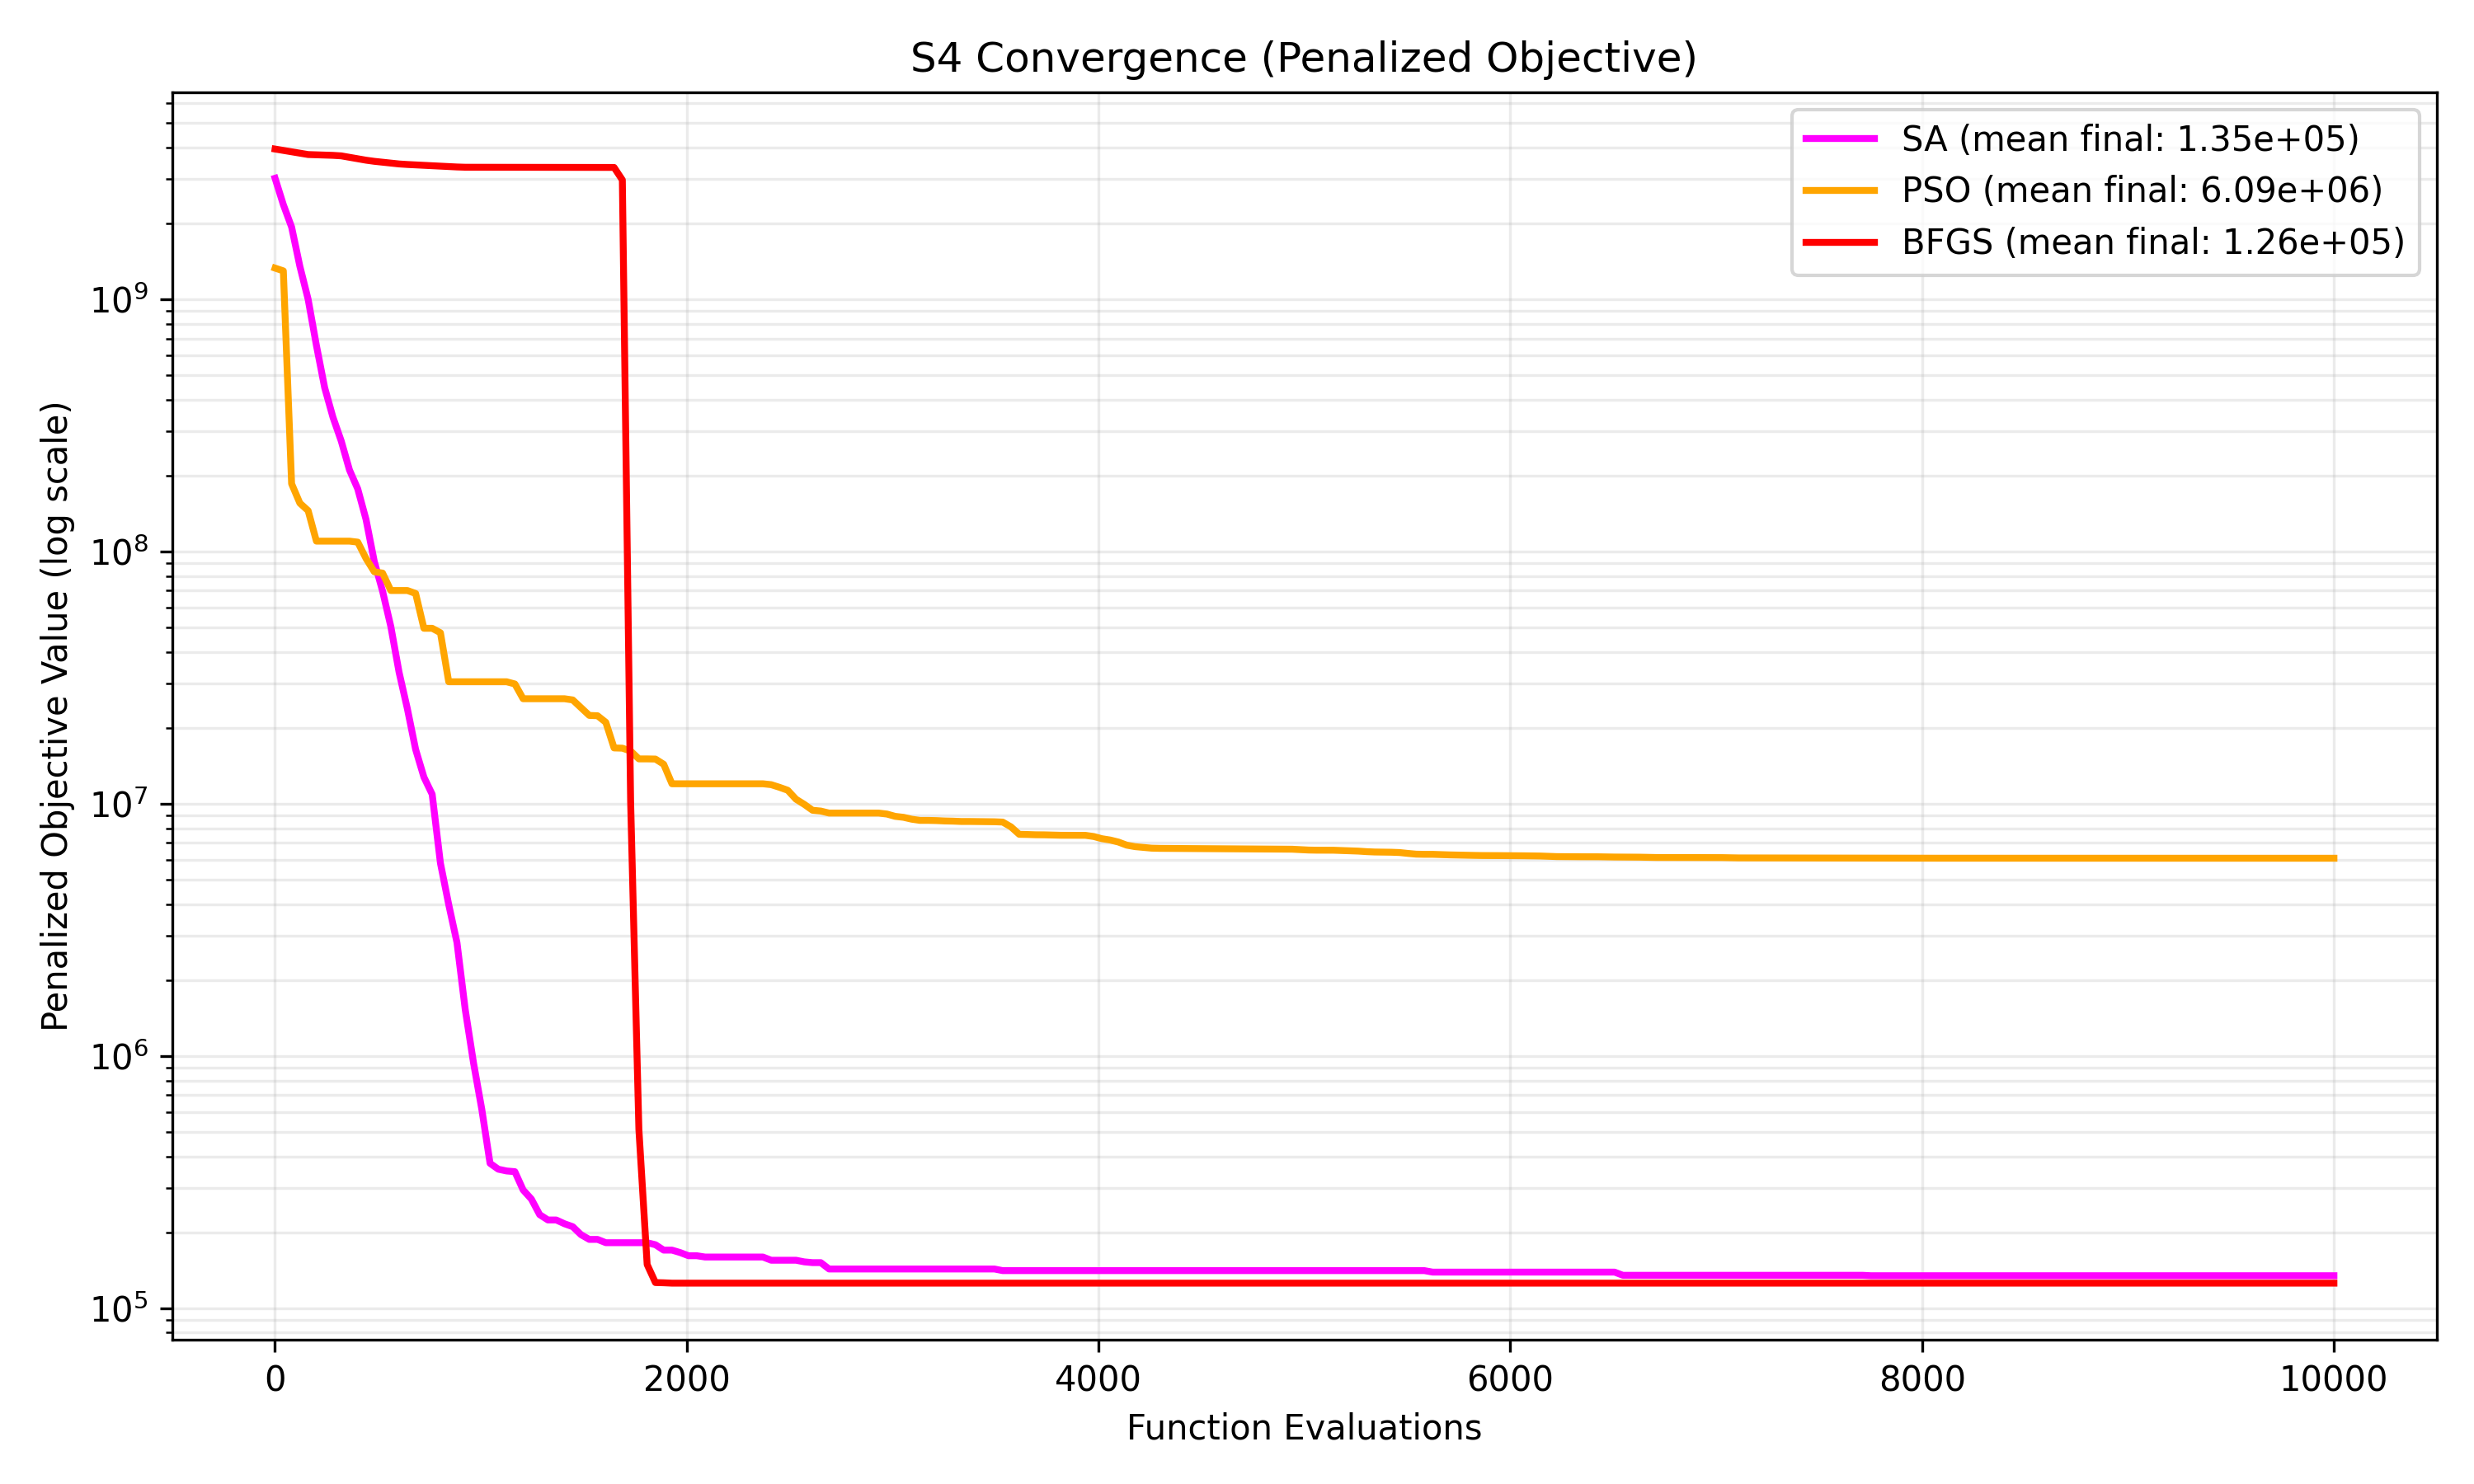
\includegraphics[width=0.95\textwidth]{../results/figures/S4_convergence.png}
\caption{S4 convergence}
\end{figure}


\begin{figure}[H]
\centering
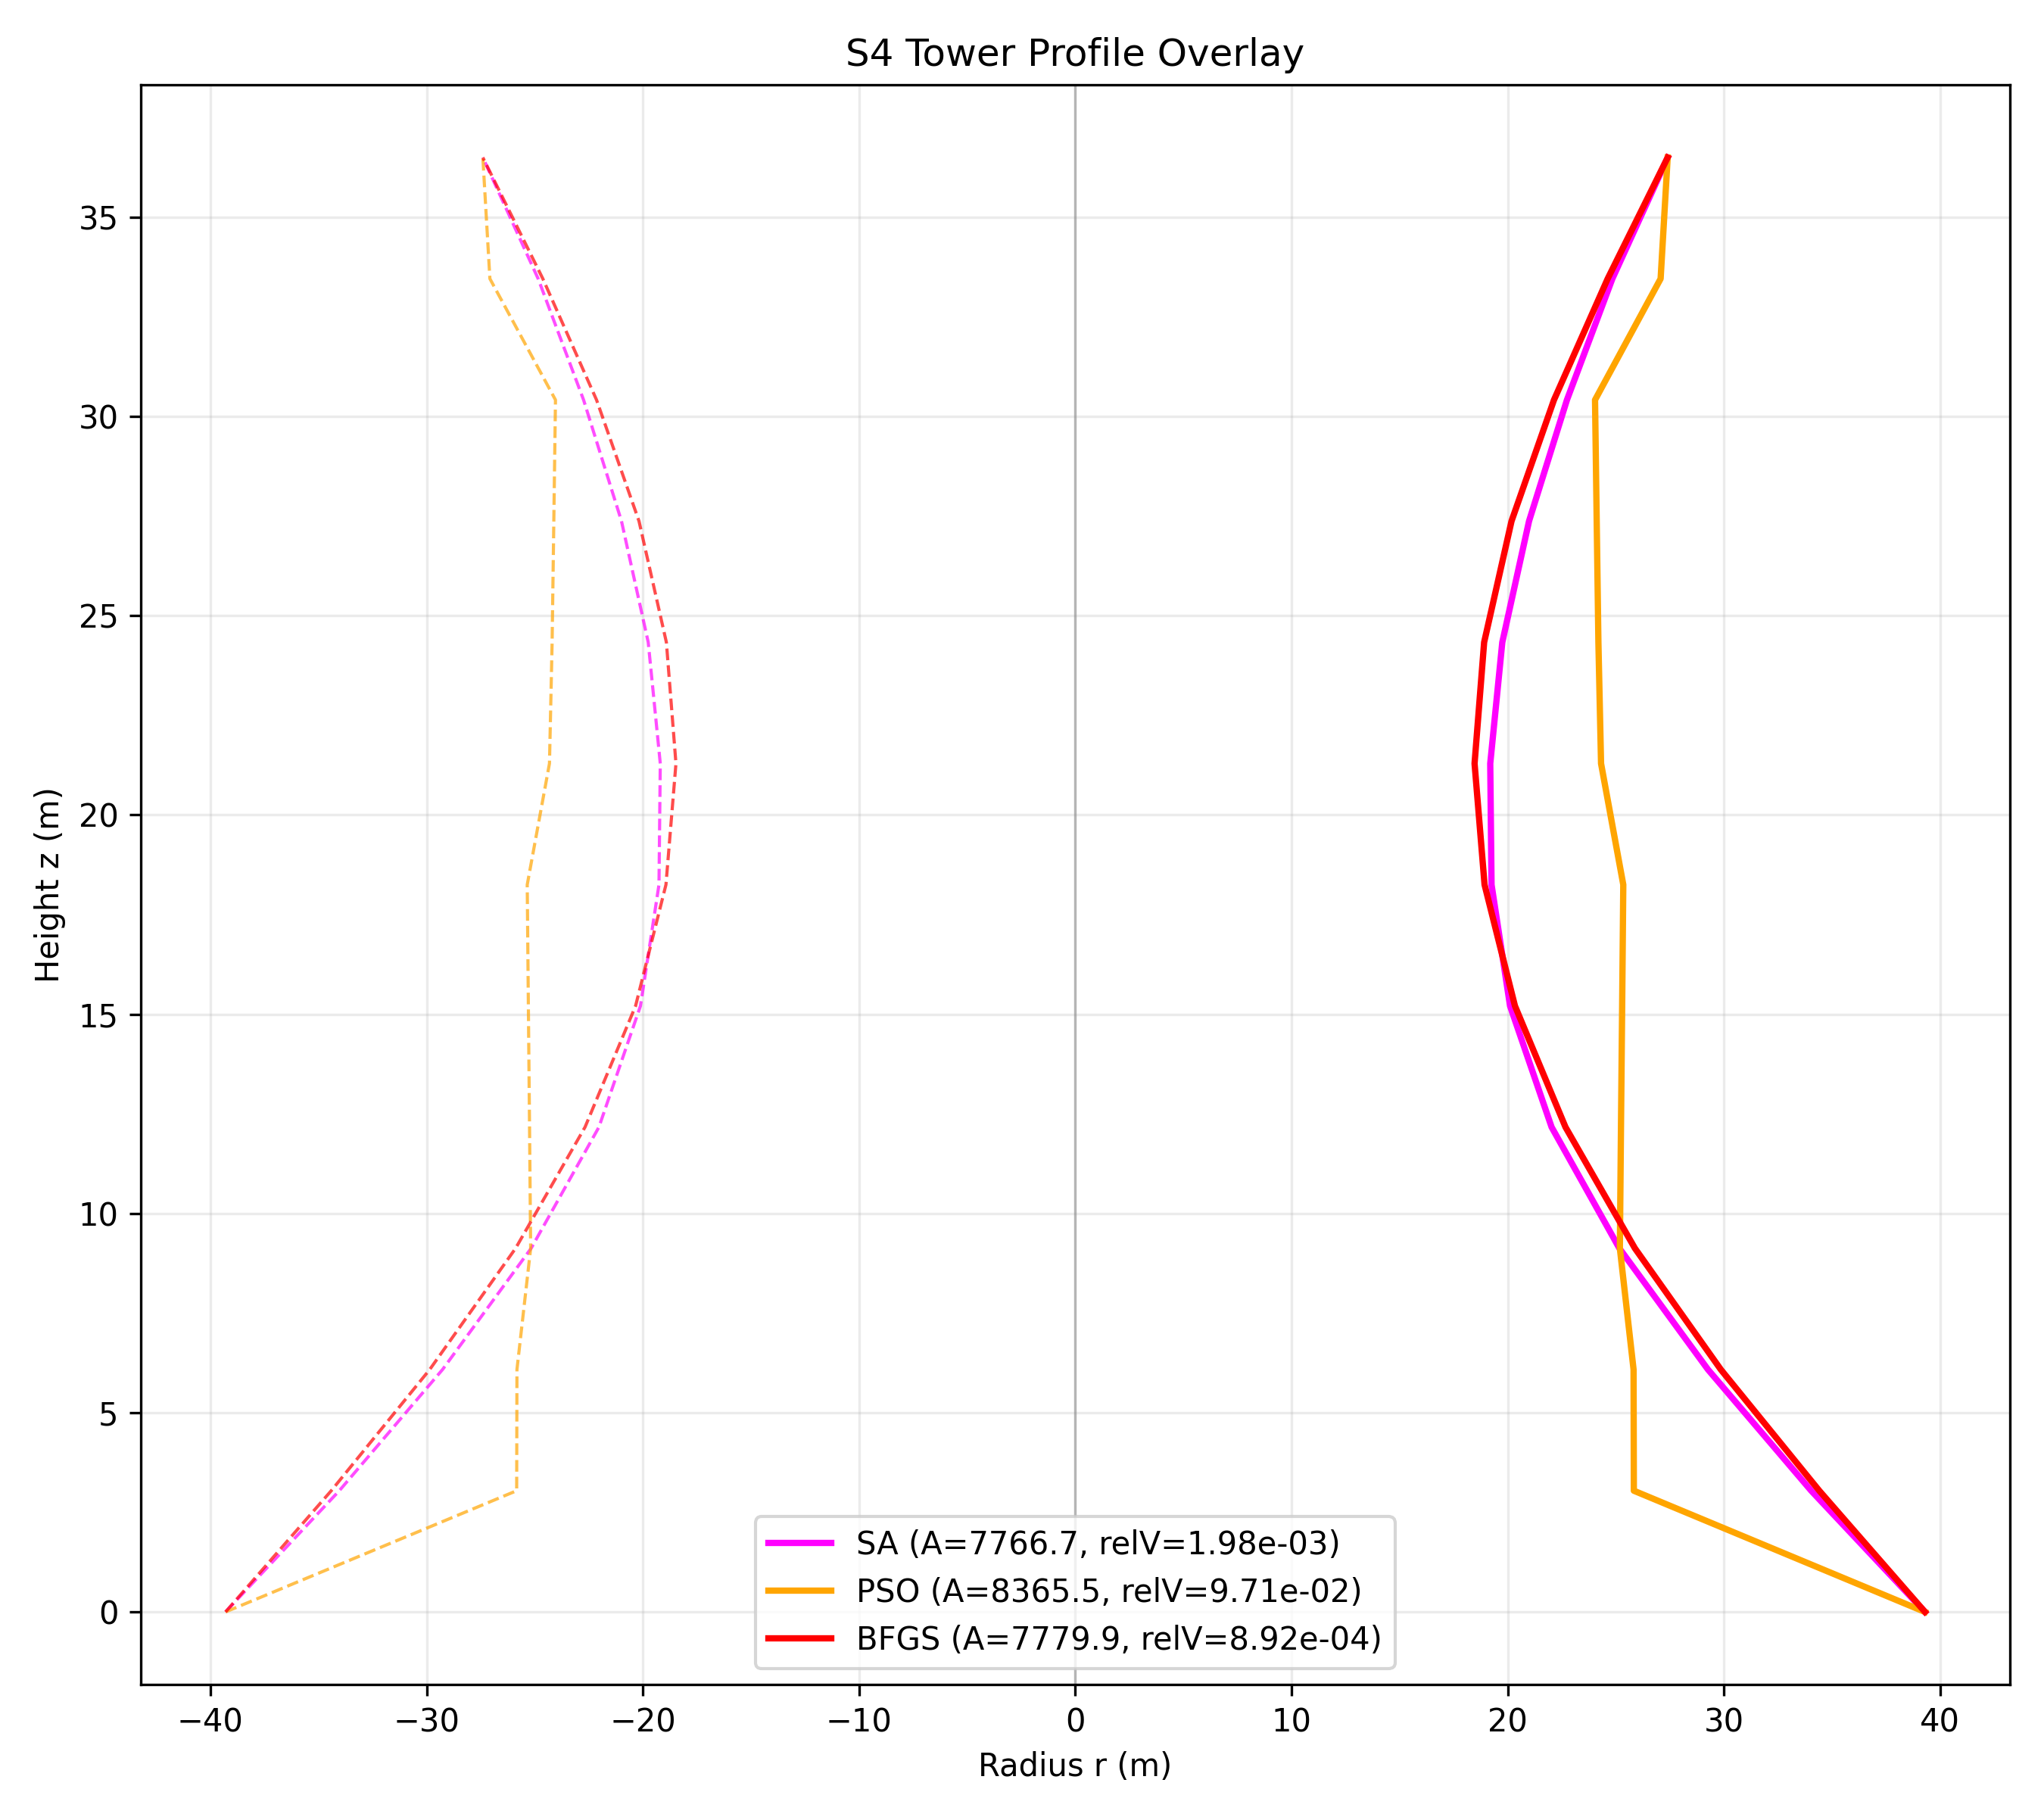
\includegraphics[width=0.95\textwidth]{../results/figures/S4_profile_overlay.png}
\caption{S4 profile}
\end{figure}


\begin{figure}[H]
\centering

\includegraphics[width=0.95\textwidth]{../results/figures/S4_tower_3d.png}
\caption{S4 3D towers}
\end{figure}



\section{S5}

\begin{longtable}{p{0.13\textwidth} | p{0.13\textwidth} | p{0.13\textwidth} | p{0.13\textwidth} | p{0.13\textwidth} | p{0.13\textwidth} | p{0.13\textwidth}}
\hline
Algorithm & Mean Area & Std Area & Mean Rel Vol Err & Mean Evals & Mean Time (s) & Feasibility Rate \\
\hline
\endfirsthead
\hline
Algorithm & Mean Area & Std Area & Mean Rel Vol Err & Mean Evals & Mean Time (s) & Feasibility Rate \\
\hline
\endhead
BFGS & 7742.56 & 0.00 & 2.331e-06 & 4164.2 & 0.1605 & 100.0\% \\
PSO & 7796.77 & 32.30 & 1.128e-04 & 10000.0 & 0.4224 & 90.0\% \\
SA & 7757.25 & 6.61 & 3.902e-05 & 10000.0 & 0.3972 & 100.0\% \\
\hline
\end{longtable}


\begin{figure}[H]
\centering
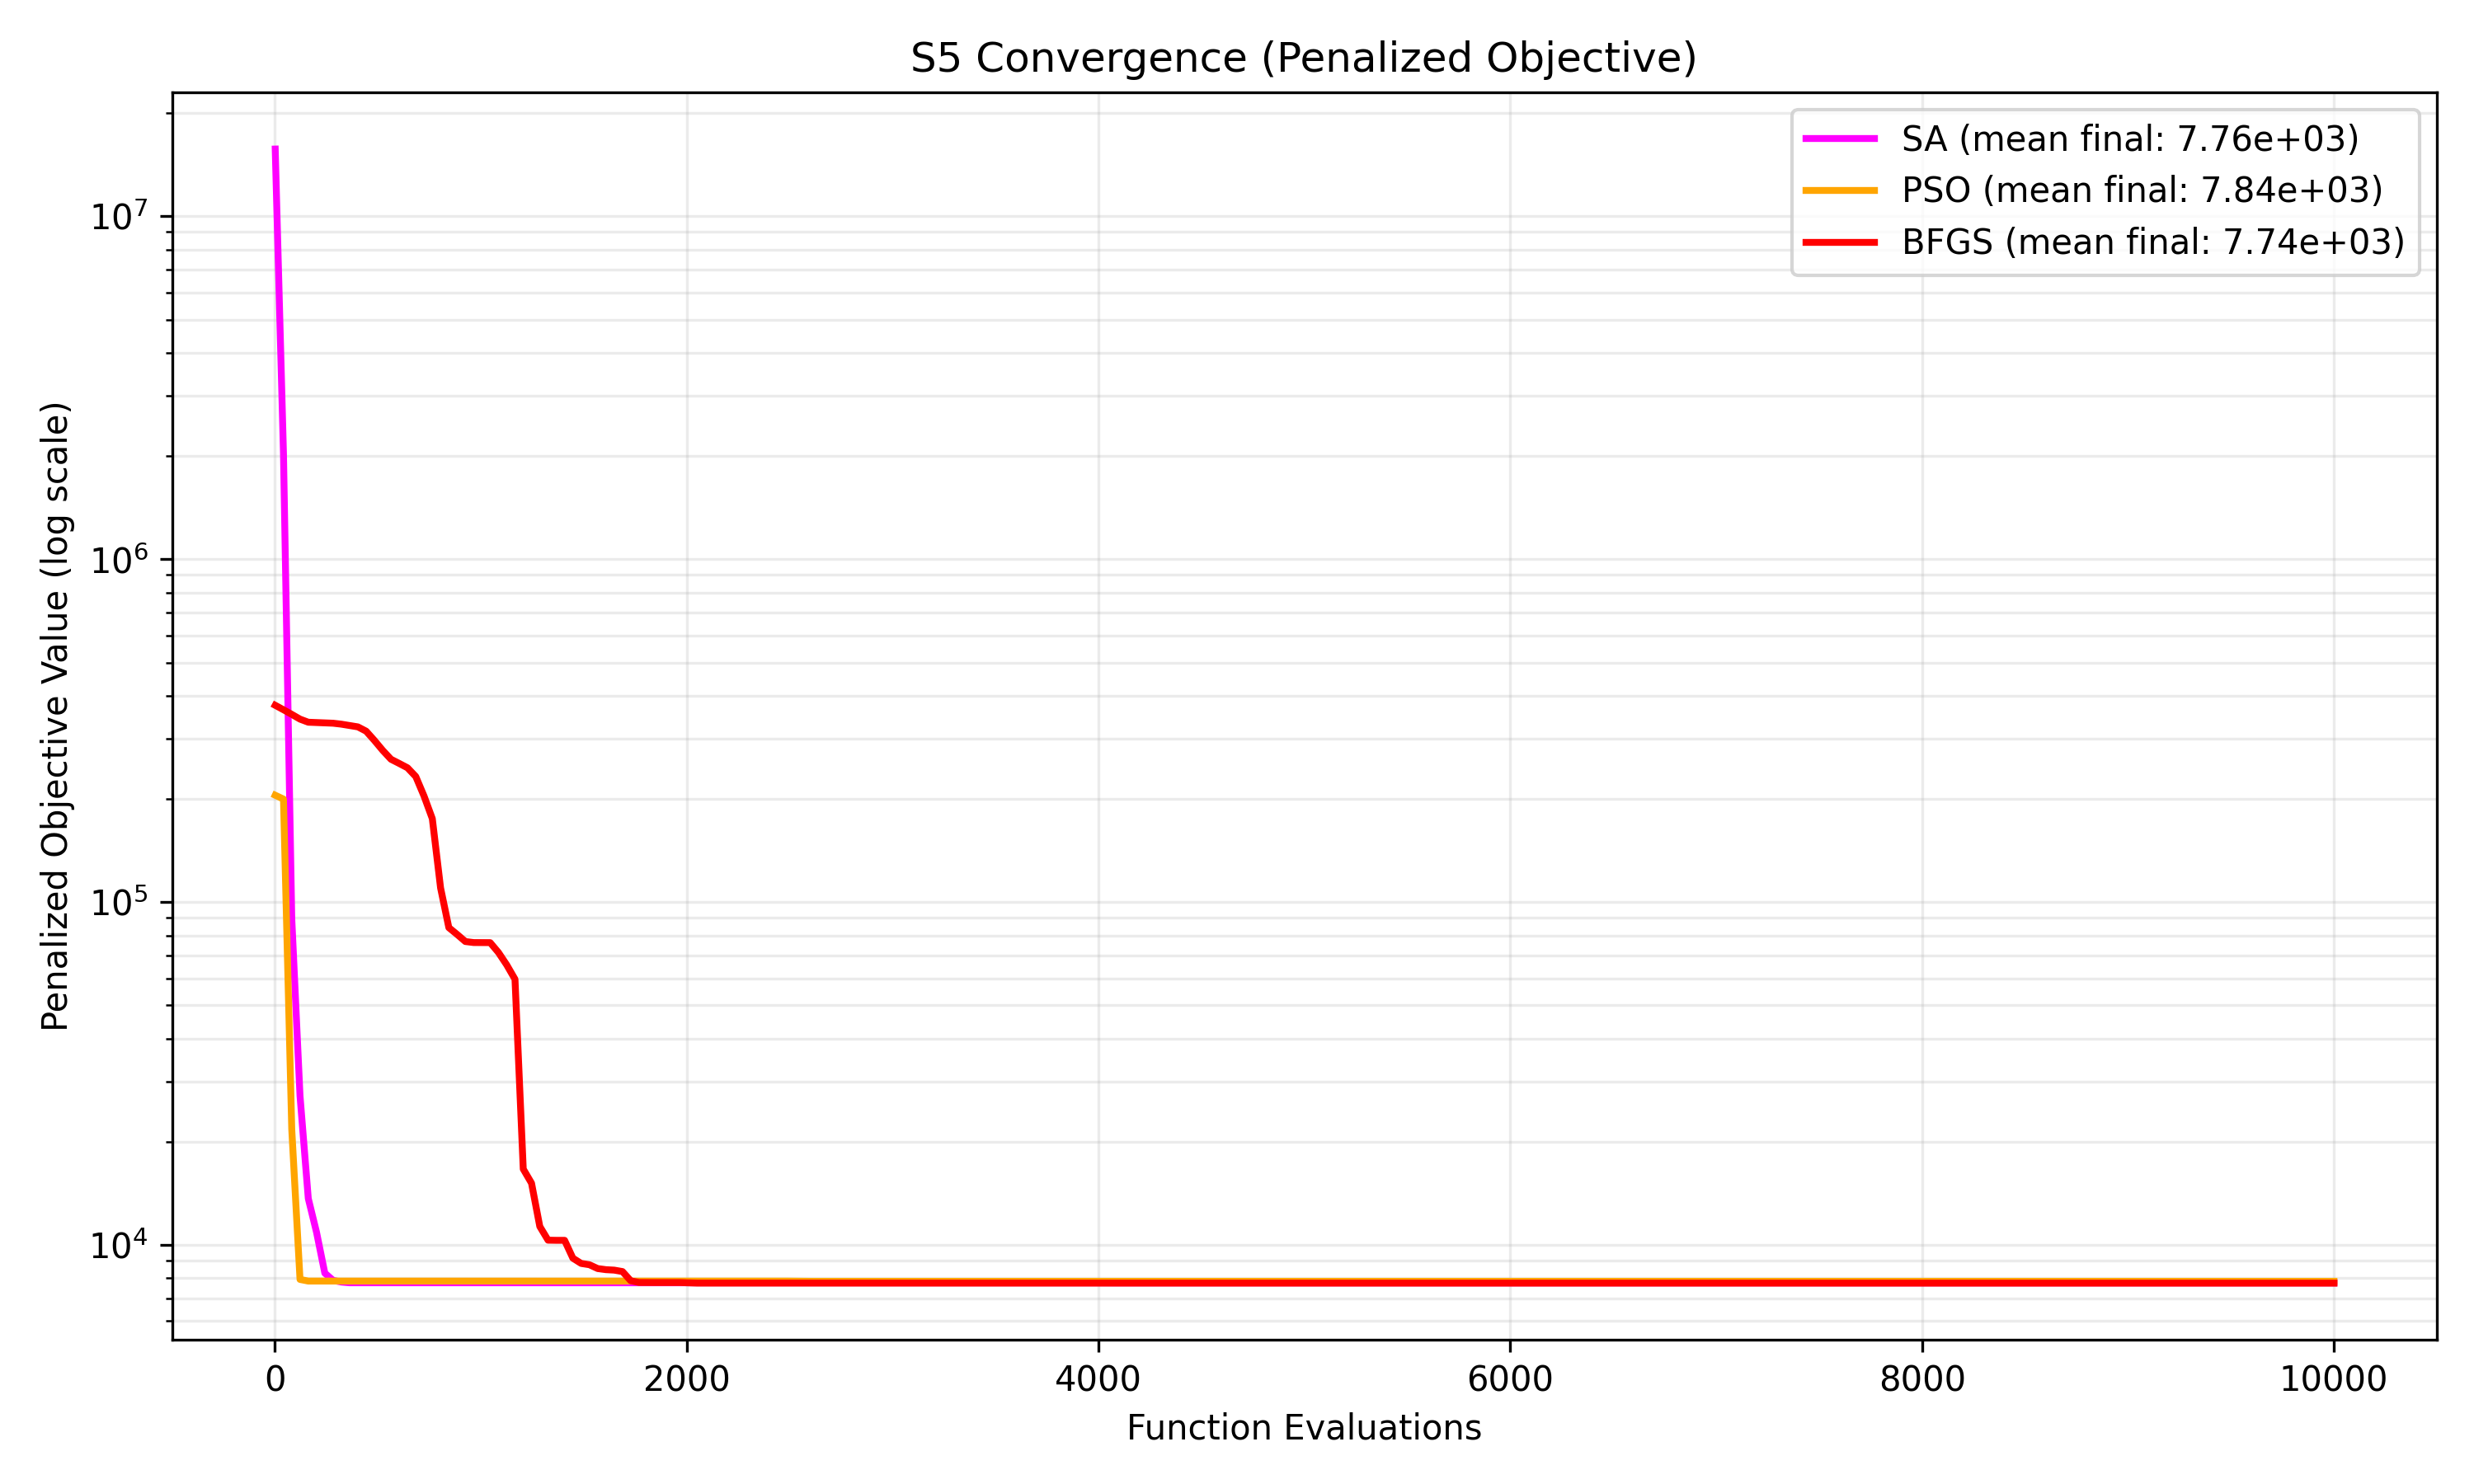
\includegraphics[width=0.95\textwidth]{../results/figures/S5_convergence.png}
\caption{S5 convergence}
\end{figure}


\begin{figure}[H]
\centering
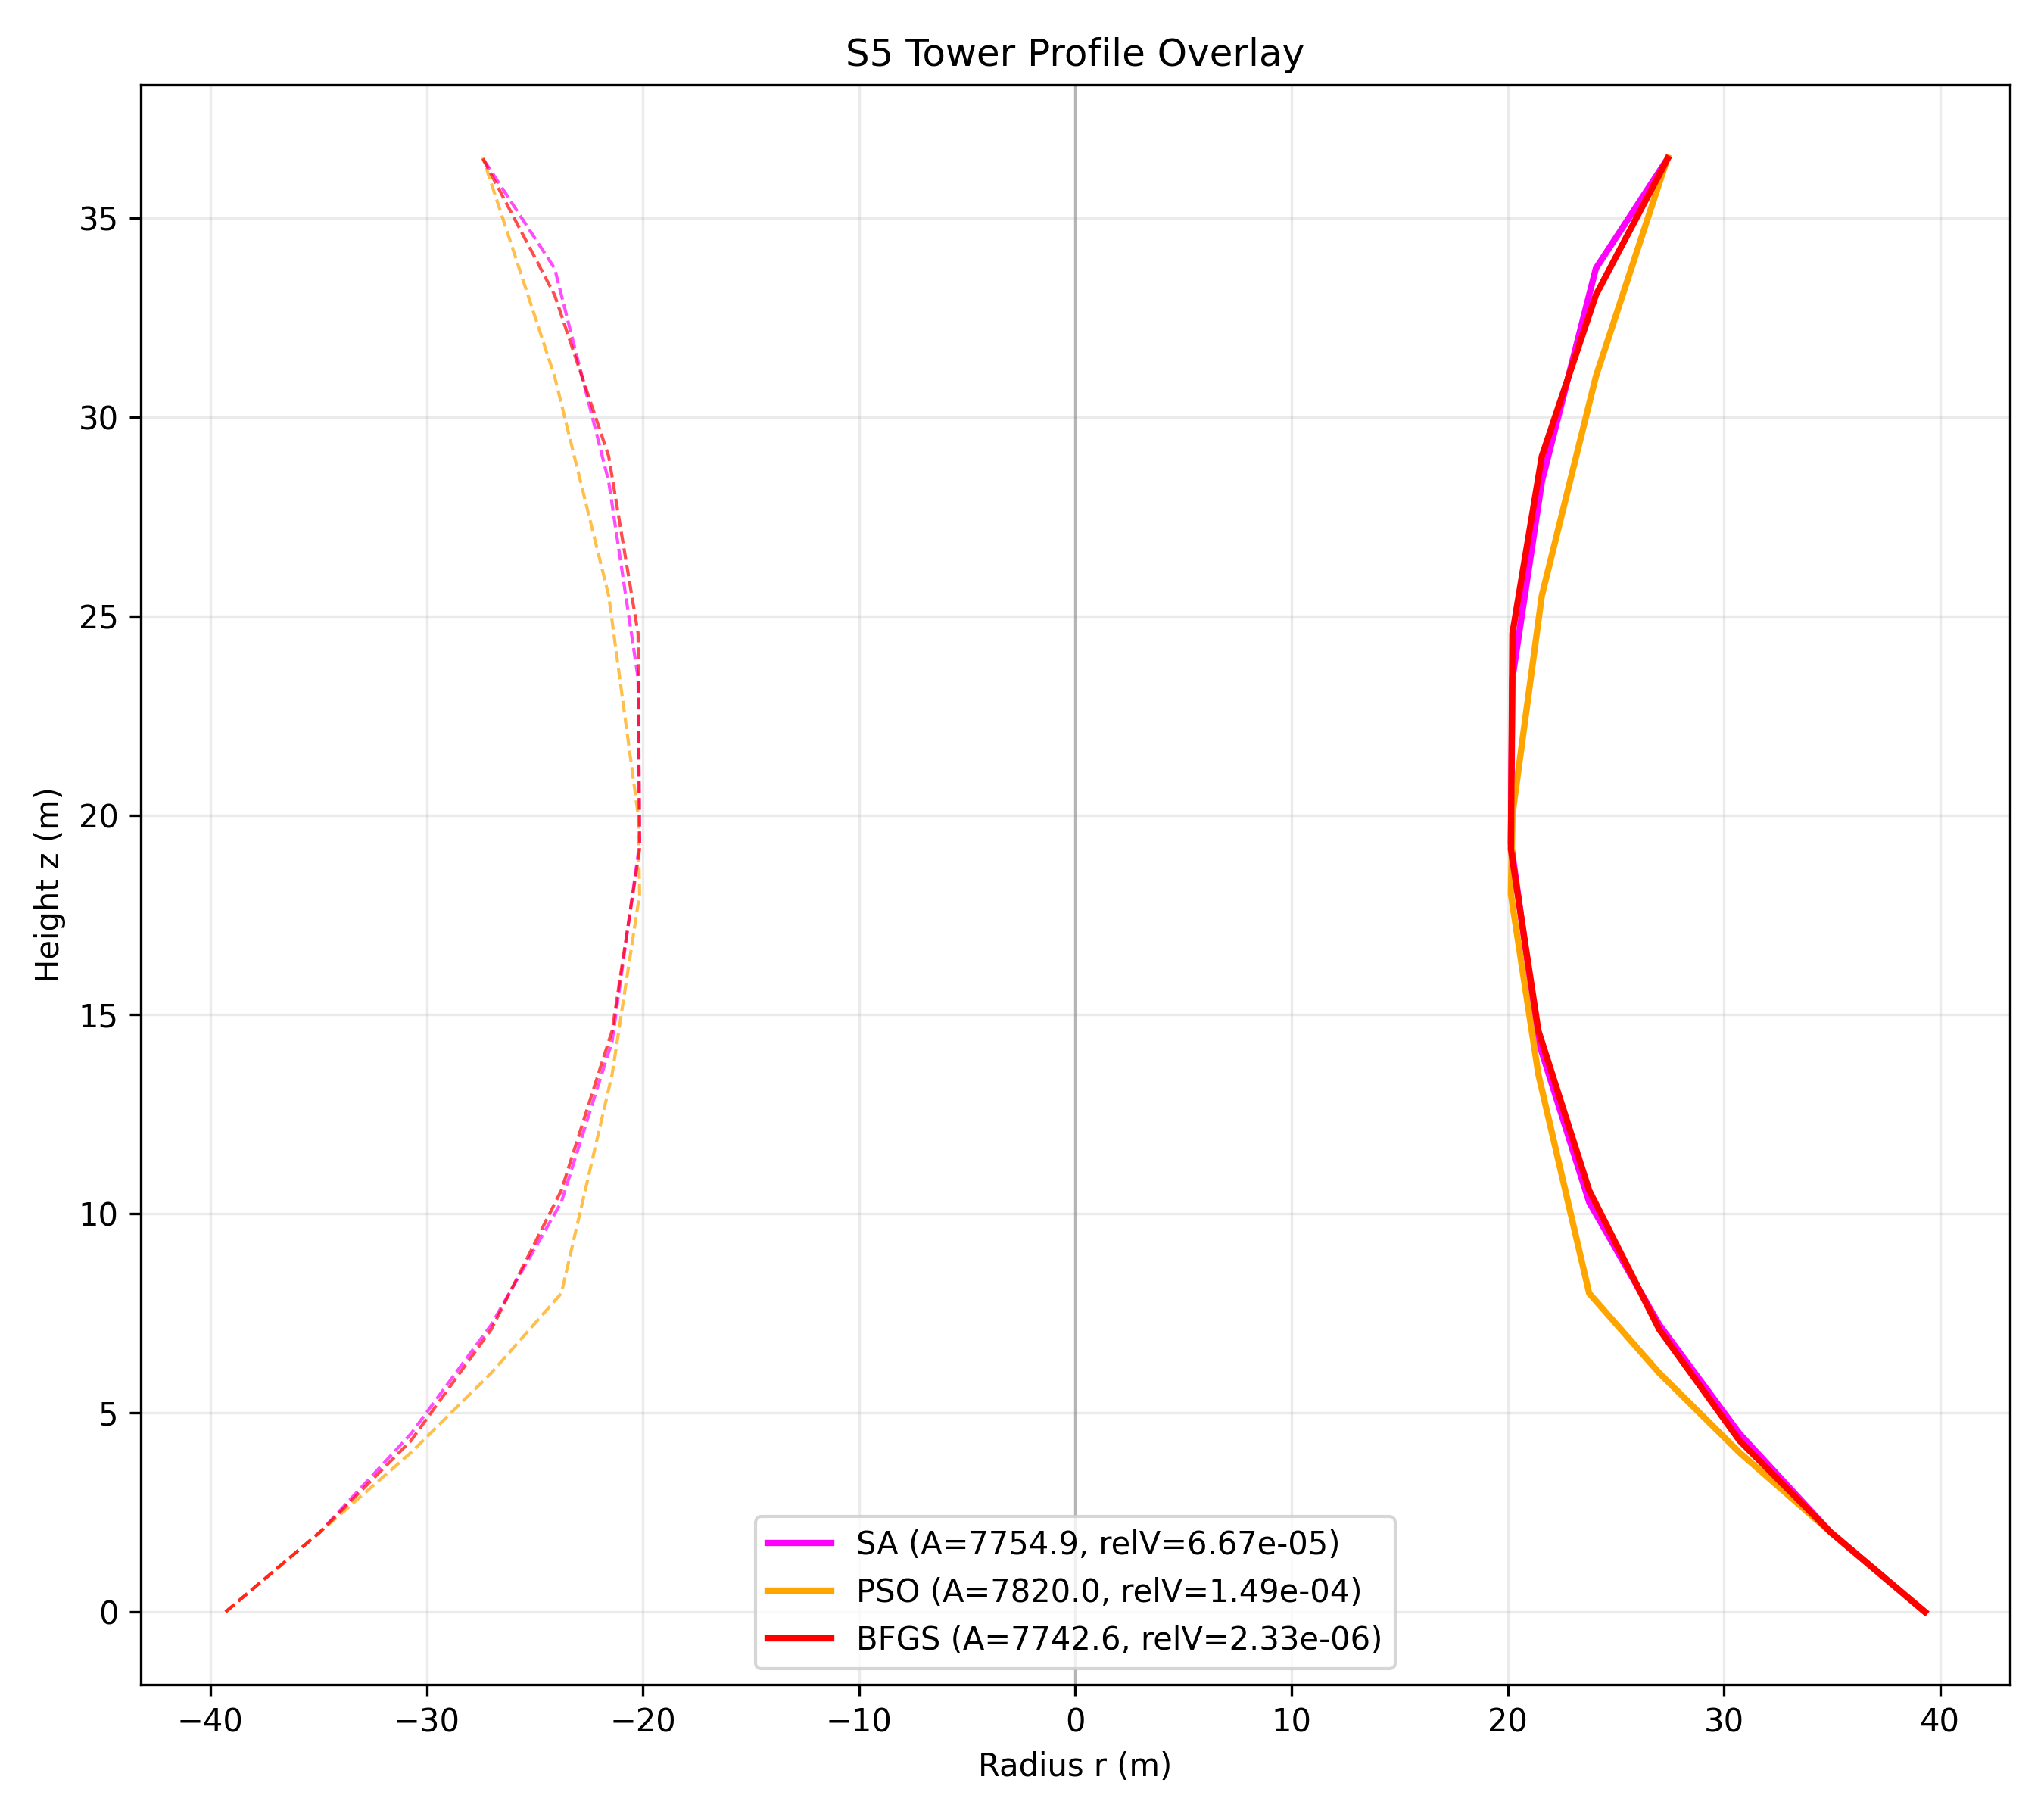
\includegraphics[width=0.95\textwidth]{../results/figures/S5_profile_overlay.png}
\caption{S5 profile}
\end{figure}


\begin{figure}[H]
\centering

\includegraphics[width=0.95\textwidth]{../results/figures/S5_tower_3d.png}
\caption{S5 3D towers}
\end{figure}



\section{S6}

\begin{longtable}{p{0.13\textwidth} | p{0.13\textwidth} | p{0.13\textwidth} | p{0.13\textwidth} | p{0.13\textwidth} | p{0.13\textwidth} | p{0.13\textwidth}}
\hline
Algorithm & Mean Area & Std Area & Mean Rel Vol Err & Mean Evals & Mean Time (s) & Feasibility Rate \\
\hline
\endfirsthead
\hline
Algorithm & Mean Area & Std Area & Mean Rel Vol Err & Mean Evals & Mean Time (s) & Feasibility Rate \\
\hline
\endhead
BFGS & 7741.72 & 0.00 & 2.071e-06 & 1402.6 & 0.0560 & 100.0\% \\
PSO & 7913.68 & 146.68 & 5.923e-04 & 10000.0 & 0.4250 & 90.0\% \\
SA & 7825.77 & 33.17 & 6.569e-05 & 10000.0 & 0.3995 & 100.0\% \\
\hline
\end{longtable}


\begin{figure}[H]
\centering

\includegraphics[width=0.95\textwidth]{../results/figures/S6_convergence.png}
\caption{S6 convergence}
\end{figure}


\begin{figure}[H]
\centering

\includegraphics[width=0.95\textwidth]{../results/figures/S6_profile_overlay.png}
\caption{S6 profile}
\end{figure}


\begin{figure}[H]
\centering

\includegraphics[width=0.95\textwidth]{../results/figures/S6_tower_3d.png}
\caption{S6 3D towers}
\end{figure}



\section{S7}

\begin{longtable}{p{0.13\textwidth} | p{0.13\textwidth} | p{0.13\textwidth} | p{0.13\textwidth} | p{0.13\textwidth} | p{0.13\textwidth} | p{0.13\textwidth}}
\hline
Algorithm & Mean Area & Std Area & Mean Rel Vol Err & Mean Evals & Mean Time (s) & Feasibility Rate \\
\hline
\endfirsthead
\hline
Algorithm & Mean Area & Std Area & Mean Rel Vol Err & Mean Evals & Mean Time (s) & Feasibility Rate \\
\hline
\endhead
BFGS & 7968.31 & 369.60 & 6.476e-05 & 7000.9 & 0.3292 & 80.0\% \\
PSO & 8608.62 & 174.56 & 4.144e-04 & 16000.0 & 0.7790 & 70.0\% \\
SA & 8160.14 & 281.40 & 1.305e-04 & 16000.0 & 0.7315 & 100.0\% \\
\hline
\end{longtable}


\begin{figure}[H]
\centering
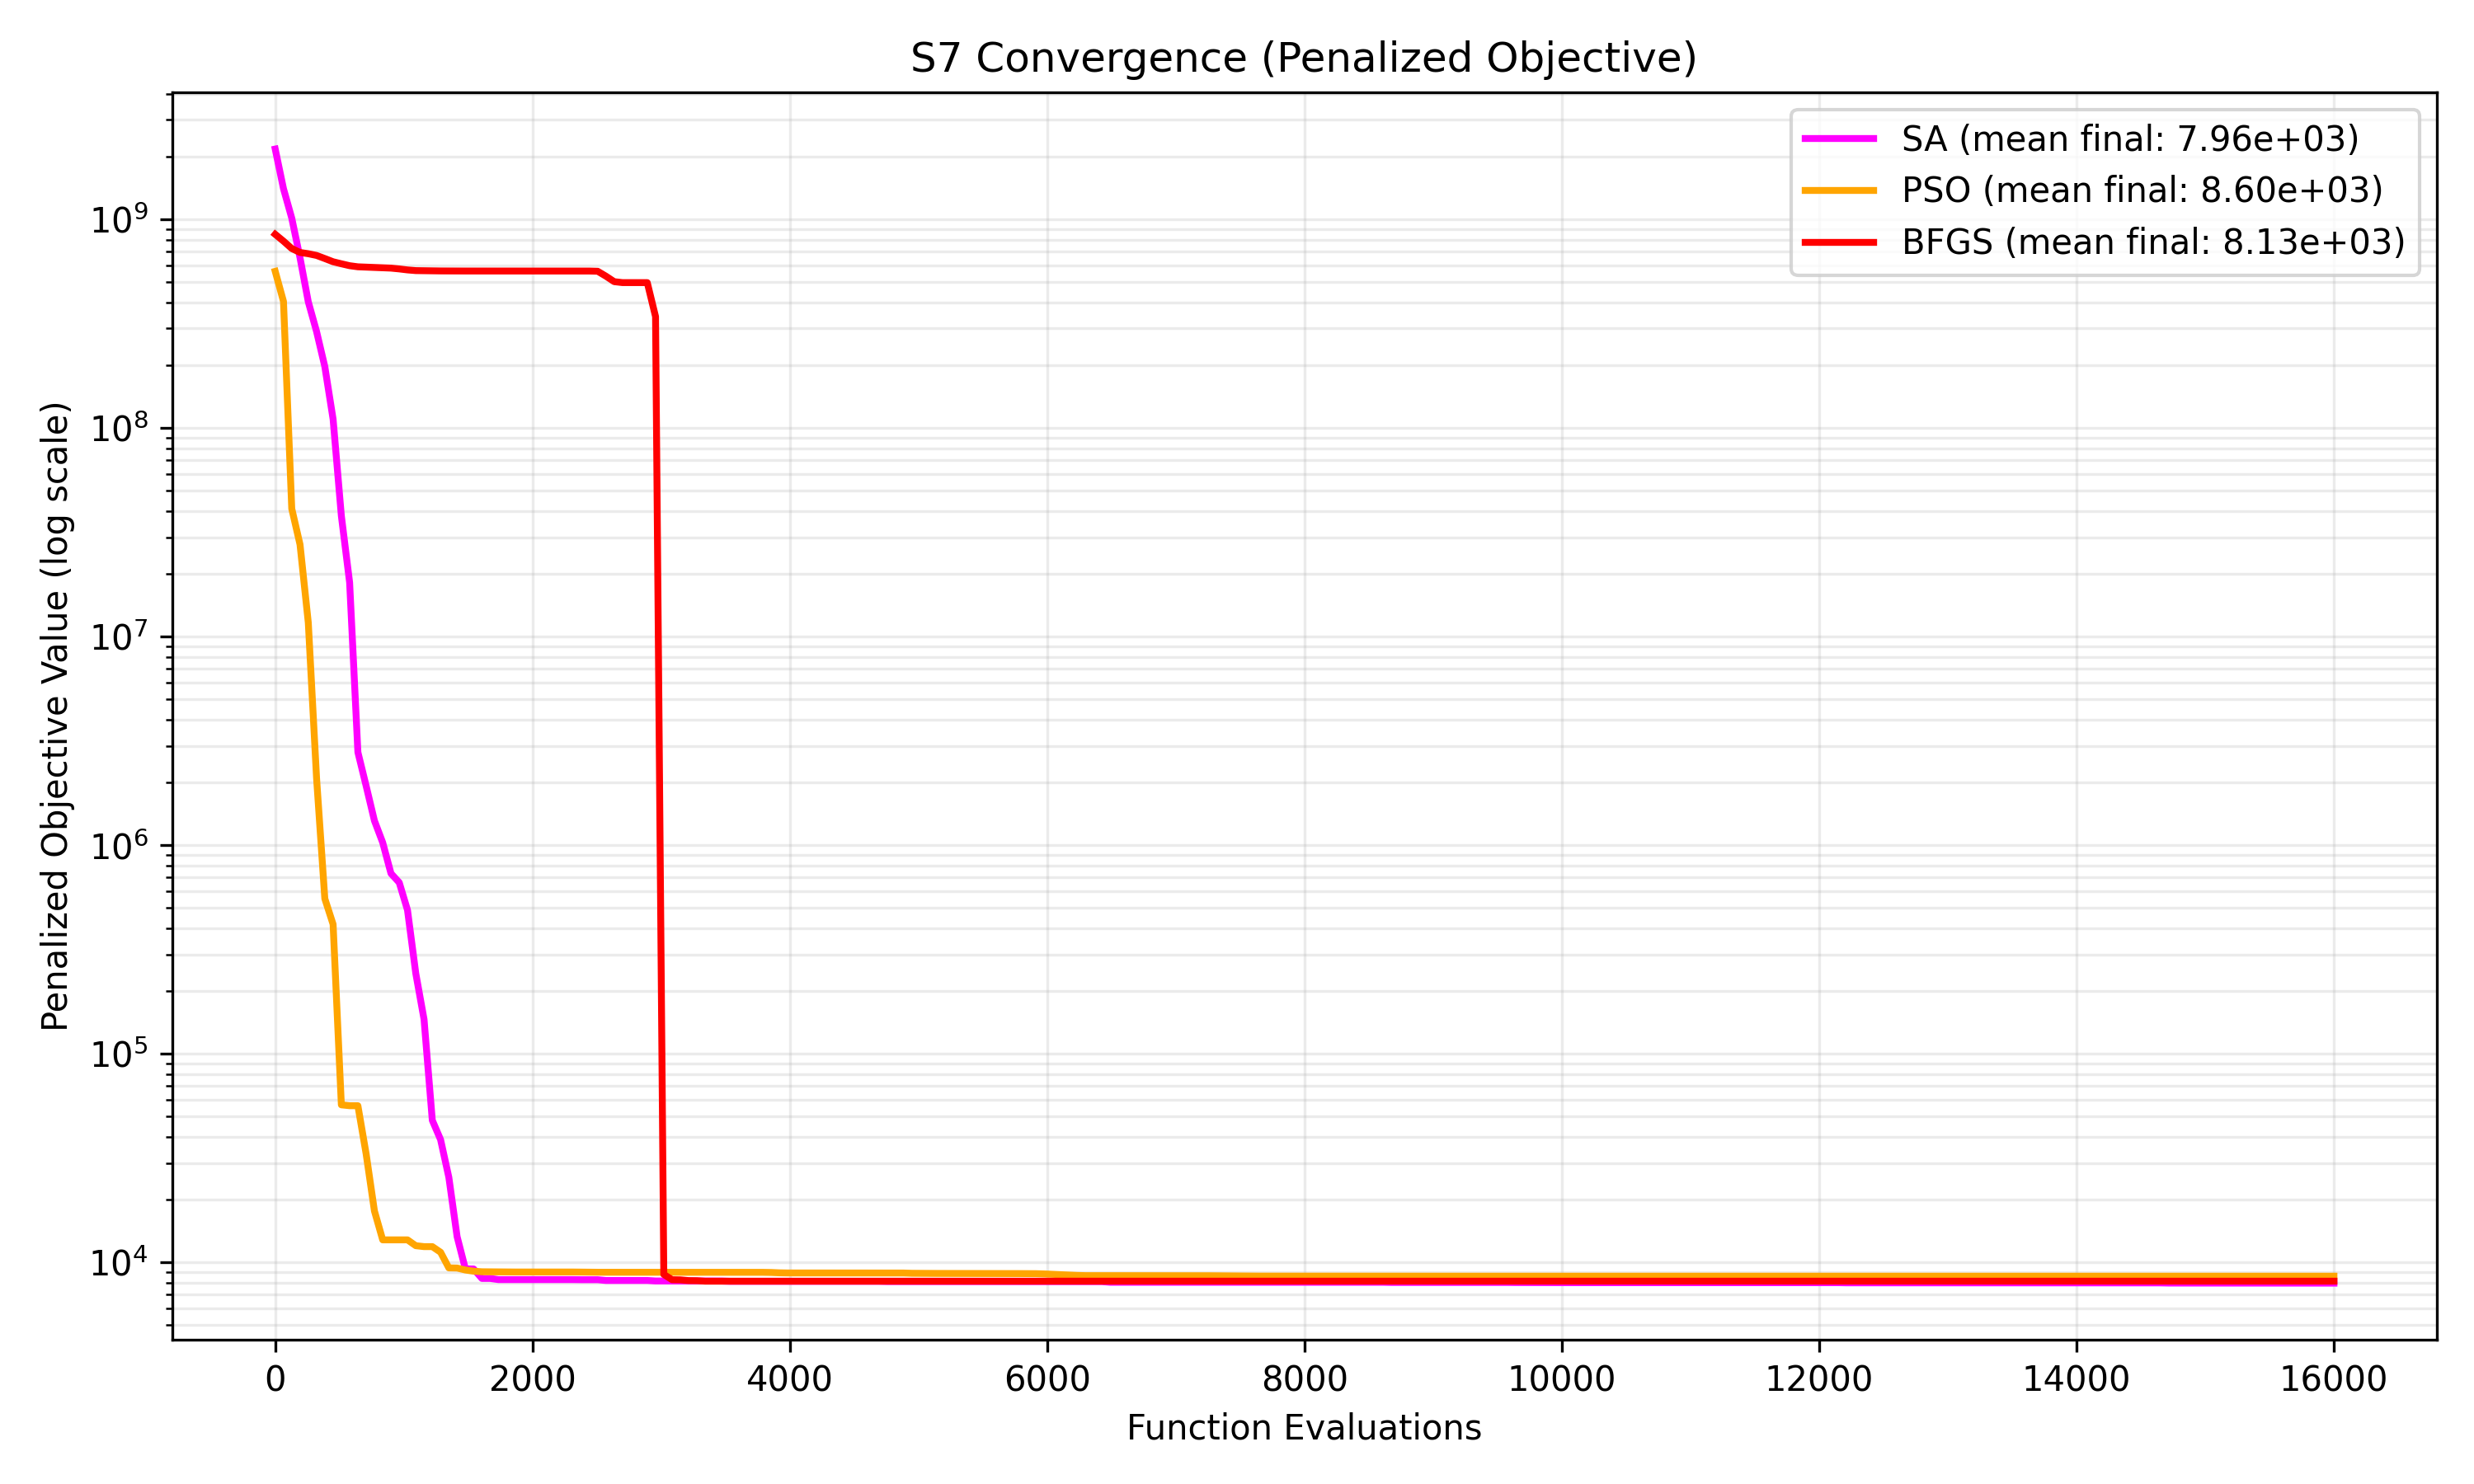
\includegraphics[width=0.95\textwidth]{../results/figures/S7_convergence.png}
\caption{S7 convergence}
\end{figure}


\begin{figure}[H]
\centering

\includegraphics[width=0.95\textwidth]{../results/figures/S7_profile_overlay.png}
\caption{S7 profile}
\end{figure}


\begin{figure}[H]
\centering

\includegraphics[width=0.95\textwidth]{../results/figures/S7_tower_3d.png}
\caption{S7 3D towers}
\end{figure}



\section{S8}

\begin{longtable}{p{0.13\textwidth} | p{0.13\textwidth} | p{0.13\textwidth} | p{0.13\textwidth} | p{0.13\textwidth} | p{0.13\textwidth} | p{0.13\textwidth}}
\hline
Algorithm & Mean Area & Std Area & Mean Rel Vol Err & Mean Evals & Mean Time (s) & Feasibility Rate \\
\hline
\endfirsthead
\hline
Algorithm & Mean Area & Std Area & Mean Rel Vol Err & Mean Evals & Mean Time (s) & Feasibility Rate \\
\hline
\endhead
BFGS & 7813.08 & 0.46 & 4.146e-04 & 7001.0 & 0.4476 & 0.0\% \\
PSO & 7968.67 & 348.77 & 2.087e-02 & 16000.0 & 1.0261 & 0.0\% \\
SA & 7701.98 & 32.24 & 1.093e-03 & 16000.0 & 0.9600 & 0.0\% \\
\hline
\end{longtable}


\begin{figure}[H]
\centering

\includegraphics[width=0.95\textwidth]{../results/figures/S8_convergence.png}
\caption{S8 convergence}
\end{figure}


\begin{figure}[H]
\centering

\includegraphics[width=0.95\textwidth]{../results/figures/S8_profile_overlay.png}
\caption{S8 profile}
\end{figure}


\begin{figure}[H]
\centering

\includegraphics[width=0.95\textwidth]{../results/figures/S8_tower_3d.png}
\caption{S8 3D towers}
\end{figure}


\chapter{9. Key Findings}


\begin{itemize}
\item S1: best feasibility-area tradeoff = SA (feasibility 50.0\%, mean area 7781.85 m\textasciicircum{}2).
\item S1: lowest mean evaluation count = BFGS (3302.6 evals).
\item S2: best feasibility-area tradeoff = SA (feasibility 100.0\%, mean area 7753.26 m\textasciicircum{}2).
\item S2: lowest mean evaluation count = BFGS (3945.5 evals).
\item S3: best feasibility-area tradeoff = SA (feasibility 100.0\%, mean area 7753.02 m\textasciicircum{}2).
\item S3: lowest mean evaluation count = BFGS (2904.7 evals).
\item S4: best feasibility-area tradeoff = BFGS (feasibility 100.0\%, mean area 7779.85 m\textasciicircum{}2).
\item S4: lowest mean evaluation count = BFGS (4101.4 evals).
\item S5: best feasibility-area tradeoff = BFGS (feasibility 100.0\%, mean area 7742.56 m\textasciicircum{}2).
\item S5: lowest mean evaluation count = BFGS (4164.2 evals).
\item S6: best feasibility-area tradeoff = BFGS (feasibility 100.0\%, mean area 7741.72 m\textasciicircum{}2).
\item S6: lowest mean evaluation count = BFGS (1402.6 evals).
\item S7: best feasibility-area tradeoff = SA (feasibility 100.0\%, mean area 8160.14 m\textasciicircum{}2).
\item S7: lowest mean evaluation count = BFGS (7000.9 evals).
\item S8: best feasibility-area tradeoff = SA (feasibility 0.0\%, mean area 7701.98 m\textasciicircum{}2).
\item S8: lowest mean evaluation count = BFGS (7001.0 evals).
\end{itemize}

\begin{itemize}
\item Feasibility bottleneck scenarios: S8 (all tested methods yielded 0\% feasible runs under current constraints).
\end{itemize}

\chapter{10. Discussion and Conclusions}


Across all scenarios, \textbackslash{}textbf\{BFGS\} achieved the highest overall feasibility (72.5\%).

\textbackslash{}textbf\{BFGS\} required the fewest evaluations on average (4227.9), confirming its efficiency for local convergence.

By raw mean area across all runs, \textbackslash{}textbf\{SA\} produced the lowest average shell area (7814.56 m\textasciicircum{}2), but this must be interpreted jointly with feasibility rates.


Result patterns are consistent with expected method behavior: BFGS is computationally efficient and strong when gradients and local curvature align with feasible basins; SA is often robust under hard nonlinear penalties because probabilistic acceptance helps transition between constrained basins; PSO explores broadly but can underperform feasibility when penalty landscapes are steep and high-dimensional.


For practical engineering usage in this problem family, the recommended workflow is a hybrid strategy: use SA/PSO for global search and feasibility discovery, then warm-start BFGS for rapid refinement of the best feasible candidate.


Scenario S8 remains the principal bottleneck under the current penalty/budget setup; this indicates that constructability and enlarged-volume requirements are jointly tight. Future refinement should focus on adaptive penalty scheduling, better initialization heuristics for joint variables, and potentially increased stochastic budget for S8.


\chapter{11. Deliverables}

\begin{itemize}
\item \texttt{results/raw\_runs.csv}
\item \texttt{results/scenario\_summary.csv}
\item \texttt{results/algorithm\_summary.csv}
\item \texttt{results/scenario\_definitions.json}
\item \texttt{results/figures/*.png}
\end{itemize}
